\documentclass[border=8pt]{standalone}
\usepackage{tikz}
\usetikzlibrary{arrows.meta,positioning,calc,fit}
\begin{document}
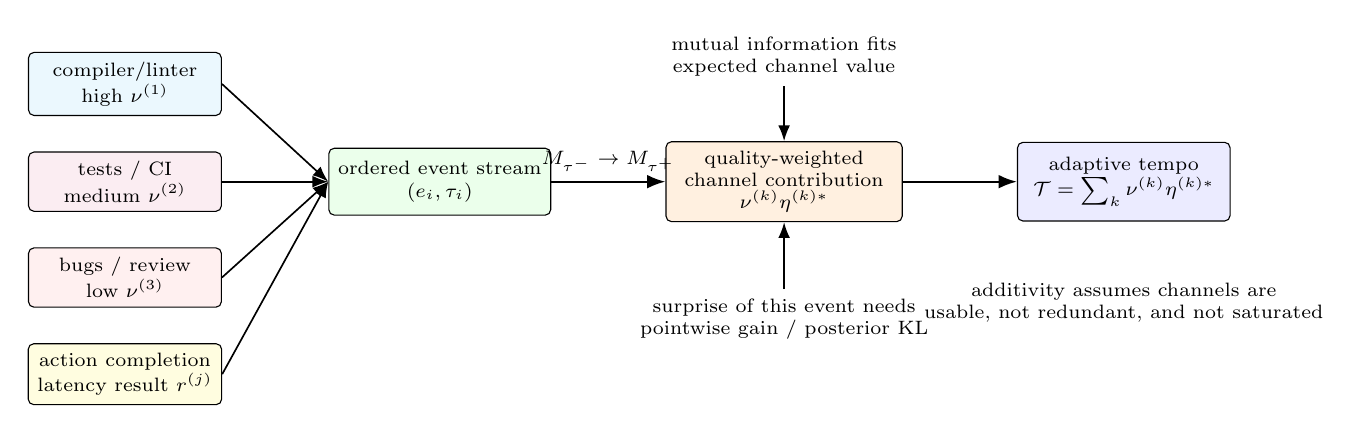
\begin{tikzpicture}[
  lane/.style={draw, rounded corners=2pt, align=center, minimum width=2.45cm, minimum height=0.72cm, font=\scriptsize},
  eventbox/.style={draw, rounded corners=2pt, align=center, minimum width=2.35cm, minimum height=0.85cm, font=\scriptsize, fill=green!8},
  bottleneck/.style={draw, rounded corners=2pt, align=center, minimum width=3.0cm, minimum height=1.0cm, font=\scriptsize, fill=orange!12},
  result/.style={draw, rounded corners=2pt, align=center, minimum width=2.7cm, minimum height=1.0cm, font=\scriptsize, fill=blue!8},
  note/.style={align=center, font=\scriptsize},
  arr/.style={-Latex, thick},
  thinarr/.style={-Latex, semithick}
]

\node[lane, fill=cyan!8] (obsfast) {compiler/linter\\high $\nu^{(1)}$};
\node[lane, fill=purple!7, below=0.45cm of obsfast] (obsmed) {tests / CI\\medium $\nu^{(2)}$};
\node[lane, fill=red!6, below=0.45cm of obsmed] (obsslow) {bugs / review\\low $\nu^{(3)}$};
\node[lane, fill=yellow!12, below=0.45cm of obsslow] (act) {action completion\\latency result $r^{(j)}$};

\node[eventbox, right=1.35cm of obsmed] (stream) {ordered event stream\\$(e_i,\tau_i)$};
\draw[thinarr] (obsfast.east) -- (stream.west);
\draw[thinarr] (obsmed.east) -- (stream.west);
\draw[thinarr] (obsslow.east) -- (stream.west);
\draw[thinarr] (act.east) -- (stream.west);

\node[bottleneck, right=1.45cm of stream] (weight) {quality-weighted\\channel contribution\\$\nu^{(k)}\eta^{(k)\ast}$};
\node[result, right=1.45cm of weight] (tempo) {adaptive tempo\\$\mathcal T=\sum_k\nu^{(k)}\eta^{(k)\ast}$};

\draw[arr] (stream) -- node[above, font=\scriptsize] {$M_{\tau^-}\to M_{\tau^+}$} (weight);
\draw[arr] (weight) -- (tempo);

\node[note, above=0.7cm of weight] (expected) {mutual information fits\\expected channel value};
\node[note, below=0.85cm of weight] (realized) {surprise of this event needs\\pointwise gain / posterior KL};
\draw[thinarr] (expected) -- (weight);
\draw[thinarr] (realized) -- (weight);

\node[note, below=0.65cm of tempo] {additivity assumes channels are\\usable, not redundant, and not saturated};

\end{tikzpicture}
\end{document}
